\documentclass[border=2pt]{standalone}
\usepackage{tikz}
\usetikzlibrary{quotes,angles}
\usepackage{amsmath}
\usepackage{amssymb}
\usepackage{babel}

\begin{document}

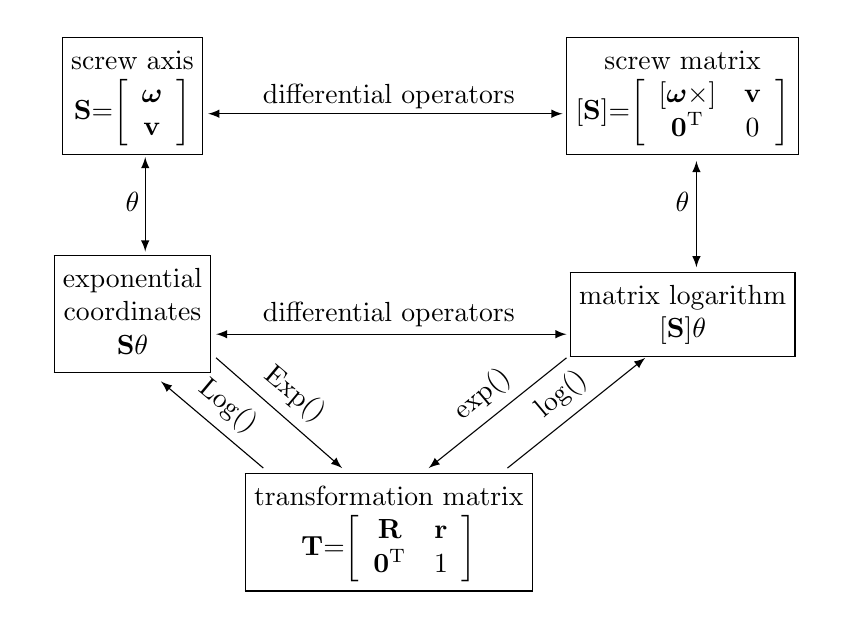
\begin{tikzpicture}[scale=1]

\node[below right] at (0.0,0.0) 
{$\begin{tabular}{ccc}
 \boxed{\begin{tabular}{@{}c@{}}
 screw axis\\
 \text{\ensuremath{\mathbf{S}}=\ensuremath{\left[\begin{array}{c}
\boldsymbol{\omega}\\
\mathbf{v}
\end{array}\right]}} 
\end{tabular}} &  differential operators  &  \boxed{\begin{tabular}{@{}c@{}}
 screw matrix\\
 \text{\ensuremath{\left[\mathbf{S}\right]}=\ensuremath{\left[\begin{array}{cc}
\left[\boldsymbol{\omega}\times\right] & \mathbf{v}\\
\mathbf{0}^{\mathrm{T}} & 0
\end{array}\right]}}
\end{tabular}}\\
\\
 \text{\ensuremath{\theta}}  &   & \text{\ensuremath{\theta}}\\
\\
 \boxed{\begin{tabular}{@{}c@{}}
 exponential\\
 coordinates\\
\text{\ensuremath{\mathbf{S}}\ensuremath{\ensuremath{\theta}}}
\end{tabular}} &  differential operators  &  \boxed{\begin{tabular}{@{}c@{}}
 matrix logarithm\\
 \text{\ensuremath{\left[\mathbf{S}\right]}\ensuremath{\ensuremath{\theta}}}
\end{tabular}}\\
\\
\\
  &   &  \\
  &  \boxed{\begin{tabular}{@{}c@{}}
 transformation matrix\\
\text{\ensuremath{\mathbf{T}}=\ensuremath{\left[\begin{array}{cc}
\mathbf{R} & \mathbf{r}\\
\mathbf{0}^{\mathrm{T}} & 1
\end{array}\right]}}
\end{tabular}}  &  
\end{tabular}$};

\draw [<->,>=latex] (2.30,-1.10) -- (6.80,-1.10);
\draw [<->,>=latex] (2.40,-3.90) -- (6.85,-3.90);

\draw [<->,>=latex] (1.50,-1.65) -- (1.50,-2.85);
\draw [<->,>=latex] (8.50,-1.70) -- (8.50,-3.05);

\draw [->,>=latex] (2.40,-4.20) -- node [above, rotate=-40] {$\mathrm{Exp}()$} (4.00,-5.60);
\draw [->,>=latex] (6.85,-4.20) -- node [above, rotate= 40] {$\exp()$} (5.10,-5.60);

\draw [<-,>=latex] (1.70,-4.50) -- node [above, rotate=-40] {$\mathrm{Log}()$} (3.00,-5.60);
\draw [<-,>=latex] (7.85,-4.20) -- node [above, rotate= 40] {$\log()$} (6.10,-5.60);

\end{tikzpicture}

\end{document}

